% This is samplepaper.tex, a sample chapter demonstrating the
% LLNCS macro package for Springer Computer Science proceedings;
% Version 2.21 of 2022/01/12
%
\documentclass[runningheads]{llncs}
%
\usepackage[T1]{fontenc}
% T1 fonts will be used to generate the final print and online PDFs,
% so please use T1 fonts in your manuscript whenever possible.
% Other font encondings may result in incorrect characters.
%
\usepackage[utf8]{inputenc}
\usepackage[english]{babel}
\usepackage{booktabs}
\usepackage{hyperref}
\usepackage{graphicx}
% Used for displaying a sample figure. If possible, figure files should
% be included in EPS format.
%
\usepackage[vlined,algoruled,linesnumbered]{algorithm2e}
\usepackage{amsmath,amssymb,nccmath,mathtools}
% If you use the hyperref package, please uncomment the following two lines
% to display URLs in blue roman font according to Springer's eBook style:
\usepackage{color}
\renewcommand\UrlFont{\color{blue}\rmfamily}
\urlstyle{rm}
%
\begin{document}
%
\title{Masked Computation of the Floor Function and Its Application to the FALCON Signature}
%
\titlerunning{Masked Floor Function For FALCON}
% If the paper title is too long for the running head, you can set
% an abbreviated paper title here
%
\author{Pierre-Augustin Berthet\inst{1,3}\orcidID{0009-0005-5065-2730} \and
Justine Paillet\inst{2,3}\orcidID{0009-0009-6056-7766} \and
C\'edric Tavernier\inst{3}\orcidID{0009-0007-5224-492X}}
%
\authorrunning{P-A Berthet et al.}
% First names are abbreviated in the running head.
% If there are more than two authors, 'et al.' is used.
%
\institute{
  Télécom Paris, Palaiseau, France, \email{berthet@telecom-paris.fr}
  \and
  Université Jean-Monnet, Saint-\'Etienne, France, \email{justine.paillet@univ-st-etienne.fr}
  \and
  Hensoldt SAS FRANCE, Plaisir, France, \email{<pierre-augustin.berthet,justine.paillet,cedric.tavernier>@hensoldt.net}
}
%
\maketitle              % typeset the header of the contribution
%
\begin{abstract}
With the ongoing standardization of new POst-Quantum Cryptography (PQC) primitives by the National Institute of Standards and Technology (NIST), it is important to investigate the robustness of new designs to Side Channel Analysis (SCA). Amongst those future standards is Falcon, a lattice-based signature which relies of rational numbers. It thus requires an implementation using floating point arithmetic, which is harder to design well and secure. While recent work proposed a solution to mask the addition and the multiplication, some roadblocks remains, most noticeably how to protect the floor function. In this work we propose several methods to protect the computation of the floor function. We provide mathematical proofs of our methods as well as formal security proof in the probing model using the Non-Interference concepts. We also discuss their application to the FALCON Signature.

\keywords{Floor Function \and Floating-Point Arithmetic \and Post-Quantum Cryptography \and FALCON \and Side-Channel Analysis \and Masking}
\end{abstract}
%
%
%
\section{Introduction}
With the rise of quantum computing, mathematical problems which were hard to solve with current technologies will be easier to breach. Amongst the concerned problem is the Discrete Logarithm Problem (DLP) which can be solved in polynomial times by the Shor quantum algorithm \cite{doi:10.1137/S0036144598347011}. As much of the current asymmetric primitives rely on this problem and will be breach, new cryptographic primitves are studied. The National Institute of Standards and Technology (NIST) launched a post-quantum standardization process \cite{chen2016report}. The finalists are CRYSTALS-Kyber \cite{8406610,nistfips203mlkem}, CRYSTALS-Dilithium \cite{Ducas_Kiltz_Lepoint_Lyubashevsky_Schwabe_Seiler_Stehlé_2018,nistfips204mldsa}, SPHINCS+ \cite{10.1145/3319535.3363229,nistfips205shdsa} and FALCON \cite{prest2020falcon}.

\medskip

\noindent Another concern for the security of cryptographic primitives is their robustness to a Side-Channel opponent. Side-Channel Analysis (SCA) was first introduced by Paul Kocher \cite{10.1007/3-540-68697-5_9} in the mid-1990. This new branch of cryptanalysis focuses on studying the impact of a cryptosystem on its surroundings. AS computations take time and energy, an opponent able of accessing the variation of one or both could find correlations between its physical observations and the data manipulated, thus resulting in a leakage and a security breach. Thus, the study of weaknesses in implementations of new primitives and the ways to protect them is an active field of research.

\medskip While they have been many works focusing on CRYSTALS-Dilithium and CRYSTALS-Kyber, summed up by Ravi et al. \cite{10.1145/3603170}, FALCON is noticeably harder to protect. Indeed, the algorithm relies on floating-point arithmetic, for which there is little litterature on how to protect it.

\subsubsection{Related Work} Previous works have identified two main weaknesses within the signing process of Falcon : the pre-image computation and the Gaussian sampler. The pre-image computation was proved vulnerable by Karabulut and Aysu \cite{9586131} using an ElectroMagnetic (EM) attack. Their work was later improved by Guerreau et al. \cite{Guerreau_Martinelli_Ricosset_Rossi_2022}. To counter those attacks, Chen and Chen \cite{Chen_Chen_2024} propose a masked implementation of the addition and multiplication of FALCON. However, they did not delved into the second weakness of Falcon, the Gaussian sampler.\newline
The Gaussian sampler is vulnerable to timing attacks, as shown by previous work \cite{10.1007/978-3-662-53140-2_16,10.1145/3133956.3134028,cryptoeprint:2019/478,10.1145/3133956.3134023}. A isochronous design was proposed by Howe et al. \cite{10.1007/978-3-030-44223-1_4}. However, a successful single power analysis (SPA) was proposed by Guerreau et al. \cite{Guerreau_Martinelli_Ricosset_Rossi_2022} and further improved by Zhang et al. \cite{10.1007/978-3-031-30634-1_19}. There is currently no masking countermeasure for FALCON's Gaussian Sampler. Existing work \cite{10.1007/978-3-031-07082-2_9} tends to re-write the Gaussian Sampler to remove the use of floating arithmetic, thus avoiding the challenge of masking the floor function. 

\subsubsection{Our Contribution}
In this work we further expand the countermeasure from Chen and Chen \cite{Chen_Chen_2024} and apply it to the Gaussian Sampler. We propose a masking method based on the mantissa truncation to compute the floor function. We also propose a generic method to arithmetize the computation of the floor function. We discuss the application of both methods to masking FALCON.

\medskip

Relying on the previous work of Chen and Chen \cite{Chen_Chen_2024}, we also verify the higher-order security of our method in the probing model. Our formal proofs rely on the Non-Interference (NI) security model first introduced by Barthe et al. \cite{10.1145/2976749.2978427}.

\medskip

Finally, we provide some performances of our methods and compare them with the reference unmasked implementation and the previous work of Chen and Chen \cite{Chen_Chen_2024}. The implementation is tested on a personal computer with an Intel-Core i7-11850H CPU.


\section{Notation and Background}\label{sec:background}
\subsection{Notation}
\subsection{FALCON Sign}
FALCON \cite{prest2020falcon} is a Lattice-Based signature using the GPV framework over the NTRU problem. In this paper we will focus on the Gaussian Sampler used in the signature algorithm. For more details on the key generation or the verification, please refer to the reference paper \cite{prest2020falcon}.

\subsubsection{Signature} The signature follows the Hash-Then-Sign strategy. The message $m$ is salted with a random value $r$ and then hashed into a challenge $c$. The remainder of the signature aims at building an instance of the SIS problem upon $c$ and a public key $h$, \emph{id est} finding $\vec{s} =(s_1,s_2)$ such as $s_1 + s_2 h = c$. To do so, the need to compute $\vec{s} = (\vec{t}-\vec{z})\mathbf{B}$, with $\vec{t}$ a pre-image vector and $\vec{z}$ provided by a Gaussian Sampler. Chen and Chen \cite{Chen_Chen_2024} focuses on masking the pre-image vector computation. In this work we intend to mask the Gaussian Sampler. The signature algorithm is detailled in Algorithm \ref{alg:falconsign}:

\begin{algorithm}[H]
  \caption{FALCON Sign \cite{prest2020falcon}}
  \label{alg:falconsign}
\end{algorithm}

\subsubsection{Gaussian Sampler}


\subsection{Floor Function}\label{subsec:floorfunction}
The floor function is defined as follows:
\begin{definition}\label{def:floorfunction}
  $\forall x \in \mathbb{R}$, the floor function of $x$, denoted by $\lfloor x \rfloor$, returns the greatest integer $z$ such as $z\leq x$.
\end{definition}
There are several ways of computing the floor function. The first one relies on floating-point arithmetic. A floating-point is composed of a sign bit, exponent bits and a mantissa \cite{kahan1996ieee}. Computing the floor function on a floating-point is performed by truncating the mantissa according to the value of the exponent and of the sign. However, while this method is fast and efficient, it requires the use of the exponent and the sign. In this work we will present a method to perform this truncation in a secure manner.

\medskip

\noindent Another way of computing the floor function is to use its associated Fourier series:\begin{equation}\label{eq:floorfourier}
  \forall x \in \mathbb{R}\backsim \mathbb{Z}, \lfloor x\rfloor = x - \frac{1}{2} + \frac{1}{\pi}\sum_{k=1}^n \frac{sin(2\pi kx)}{k},\text{ with }n\rightarrow \infty
\end{equation}
However, due to its discontinuities, Equation \ref{eq:floorfourier} suffers from the Gibbs phenomenon \cite{8e44e918-40ae-3857-bb25-dc12ccf9e7c3}, as illustrated in Figure . 
\begin{figure}[!h]
  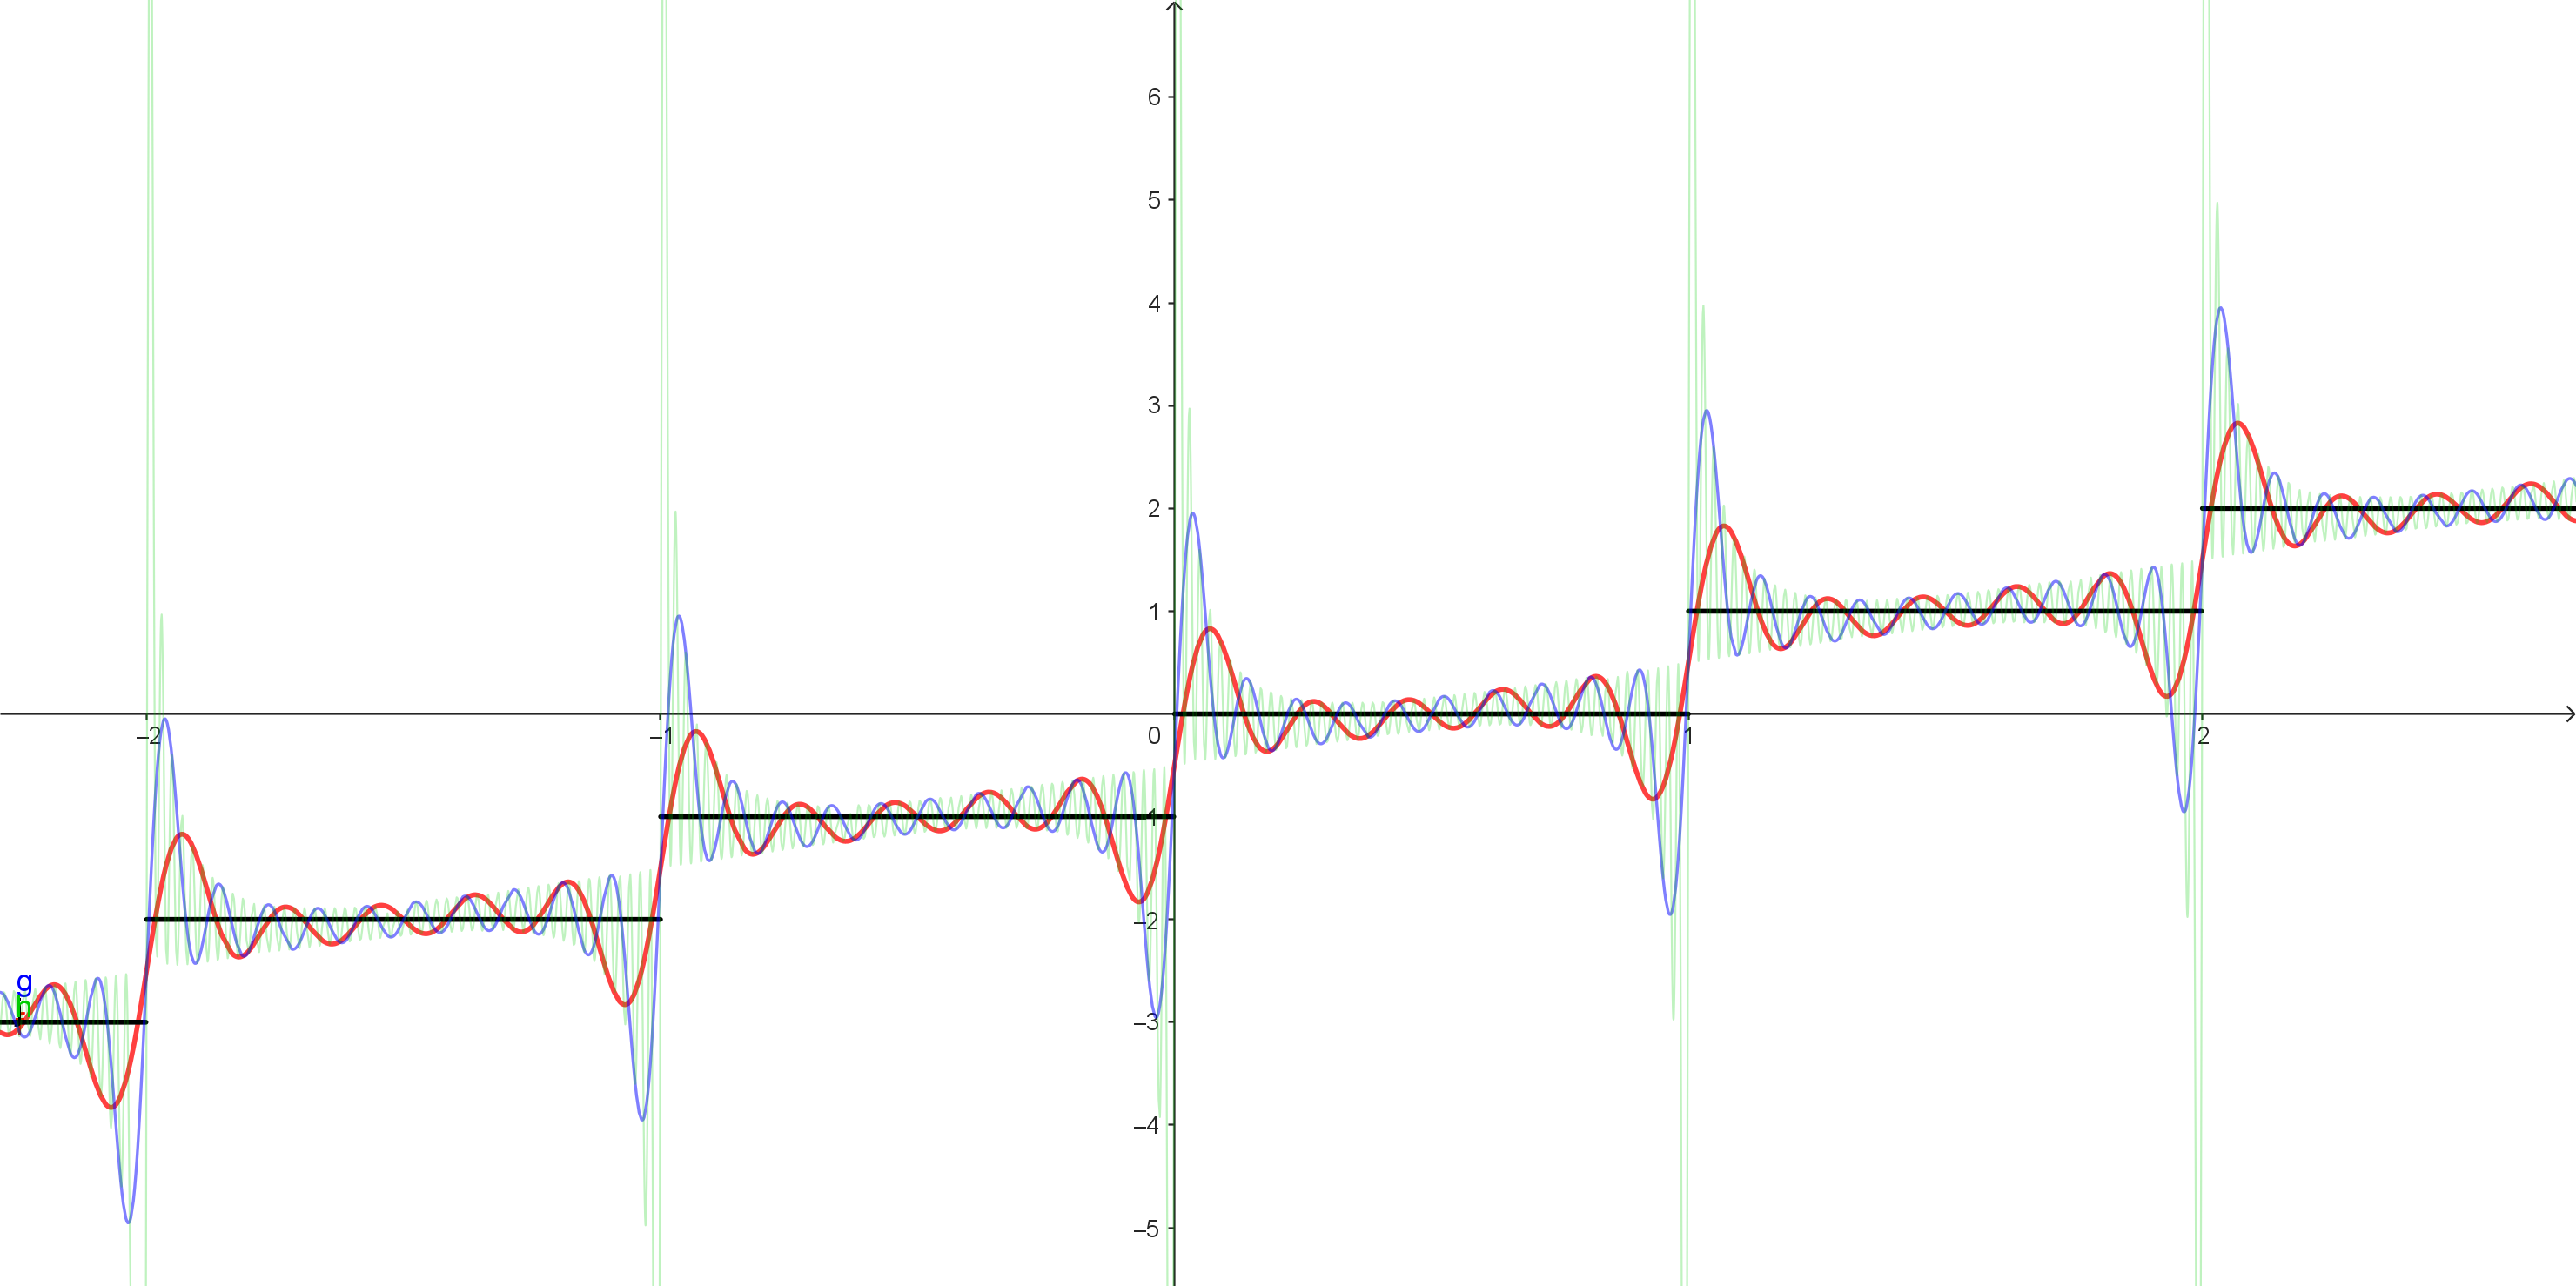
\includegraphics[width=\textwidth]{figure/gibbsphenomenon.png}
  \label{fig:gibbs}
  \caption{Gibbs phenomenon for Equation \ref{eq:floorfourier} with $n=$\textcolor{red}{5},\textcolor{blue}{10},\textcolor{green}{50} and floor(x) in black}
\end{figure}
It means this series cannot be used as it is to mask the floor function in reasonable time. Indeed, we extrapolate through empirical observations that we would require $n=2.5\times 10^{13}$ to have at least one digit of precision on the floor computation of $1\times 10^{-16}$. Nonetheless, we will see in this work how we can adapt this Fourier series to compute the floor function in a secure way and in reasonable time with the required precision.
\subsection{Masking}

\section{Masking of the Floor Function}\label{sec:maskfloor}
\subsection{Arithmetization method}
\subsubsection{Overall Strategy} The floor function can be arithmetized using Equation \ref{eq:floorfourier}. However, as stated in Section \ref{subsec:floorfunction}, this method cannot be performed in reasonable time. We thus elaborate a strategy to optimize this arithmetization.

\medskip

\noindent The first idea relies on constructing the floor of $x\in\mathbb{R}$ rather than computing it. Indeed, if we can compute the floor of $x$ with one decimal of precision, we can then multiply the result by $10$ and then reapply our computation to the new value $y=10\times \lfloor x\rfloor_1$
\subsubsection{Visual Proof}

\subsection{Truncation method}

\section{Application to FALCON}\label{sec:appfalcon}
\subsection{Masked Floor Function For FALCON}
\subsection{Masking the Gaussian Sampler}
\section{Performances}\label{sec:perf}

\section{Conclusion}\label{sec:conclusion}
\subsubsection{Acknowlegdments}

%
% ---- Bibliography ----
%
% BibTeX users should specify bibliography style 'splncs04'.
% References will then be sorted and formatted in the correct style.
%
 \bibliographystyle{splncs04}
 \bibliography{falcon}

\end{document}
